\documentclass{report}
\usepackage{graphicx}
\usepackage{fancyhdr}
\usepackage{latexsym}
\usepackage{float}
\usepackage{caption}
\usepackage{amsmath}
\usepackage{geometry}
\usepackage{tikz}
\usepackage{makecell}
\usepackage{paracol}
\usepackage{tabularx}
\setlength{\parindent}{0pt}
\geometry{a4paper,scale=0.75}
%\renewcommand\thesubsection{\arabic{subsection}}
\begin{document}
\begin{center}
    \textbf{\huge Lab Exercise \#3: Interrupt Subroutines and UART Serial Communication} \\[1em]
    Frank Li $|$
    \textbf{NetID:} jl13581 $|$
    \textbf{Email:} \texttt{jl13581@nyu.edu} $|$
    Section \textbf{C1} \\ [1em]
\end{center}
    {\Large \textbf{1. Background}}\\[0.5em]
    On our Adafruit Circuit Playground Classic board, there is one USART channel, which is USART1. Universal Asynchronous Receiver-Transmitter (UART) is a hardware communication protocol that uses asynchronous serial communication with configurable speed. It is one of the simplest and most commonly used protocols. In UART communication, data is transmitted in the form of packets, which include a start bit, data bits, an optional parity bit, and stop bits. UART does not require a clock signal, making it simpler to implement compared to synchronous communication protocols. However, it is limited by the need for both devices to agree on the baud rate and the potential for data corruption if the baud rates are not perfectly matched.\\[1em]
    {\Large \textbf{2. Experimental Procedure}}\\[0.5em]
    {\Large \textbf{2.a UART Setup}}\\[0.5em]
    For the first part of the lab, we set up the USART based on the datasheet of the microcontroller we are using, which is ATMega32U4. According to the lab manual, we know that the expected set ups are:
    \begin{center}
        \begin{tabular}{|c|c|}
        \hline
        \textbf{Parameter} & \textbf{Value} \\
        \hline
        Bit Rate & 9,600 \\
        \hline
        Data Bits & 8 \\
        \hline
        Parity & None \\
        \hline
        Stop Bits & 1 \\
        \hline
        Mode & Asynchronous/Normal Speed \\
        \hline
        \end{tabular}
    \end{center}
    Based on the above information, and the datasheet, we can set up the registers as follows:
    \begin{verbatim}
        UCSR1A = 0x00; // UCSRA set as default. 
        UCSR1B = 0x00; // UCSRB set as default.
        UCSR1C = 0x00; // UCSRC set as default.
    
        UCSR1B |= (1<<RXEN1) | // Enable receiver
                  (1<<TXEN1);  // Enable transmitter
        UCSR1C |= (1<<UCSZ10) |
                  (1<<UCSZ11); // 8-bit data
        UBRR1 = 51; // UBRR1 = (fosc / (16 * Baud Rate)) - 1
                    //       = (8MHz / (16 * 9600)) - 1 = 51.08 
    \end{verbatim}
    I first set UCSR1A, UCSR1B, and UCSR1C to zero to make sure they were set to defual before further modifications, then I set the bits RXEN1 and TXEN1 in UCSR1B to enable the receiver and transmitter, respectively. I also set the bits UCSZ10 and UCSZ11 in UCSR1C to set the data bits to 8. Finally, I set the UBRR1 register to 51 to set the baud rate to 9600. The calculation of the UBRR1 register is based on the formula given in the datasheet:
    \begin{align*}
        UBRR1 &= \frac{f_{osc}}{16 \times \text{Baud Rate}} - 1 \\
              &= \frac{8\text{MHz}}{16 \times 9600} - 1 \\
              &= 51.08
    \end{align*}
    In this case, based on the calculation result, I set the UBRR1 to 51. This code is for Team A, so the interrupt on receiver is not enabled. To enable it, we just need to add \texttt{UCSR1B |= (1<<RXCIE1)}.\\[1em]
{\Large \textbf{2.b UART Receive ISR}}\\[0.5em]
    For the second part of the lab, we set up the ISR for the USART receive interrupt. The ISR is triggered when the USART receives a byte of data. If the value is 0x31, we turn on the LED on the board. Otherwise, we turn off the LED:
\begin{verbatim}
    ISR(USART1_RX_vect){
        if (UDR1 == 0x31){
            PORTC |= (1<<PC7);
        } else{
            PORTC &= ~(1<<PC7);
        }
    }
\end{verbatim}
{\Large \textbf{2.c UART Transmit}}\\[0.5em]
    Only Team A need to transmit data to the other board, thus the transmision function is only in Team A's code. When sending values via USART, we actually directly write the value to the register UDR1. As the lab manual required, when we pressed one button (right button in our implementation), the value "0x31" will be sent. Otherwise, the value "0x30" will be sent. In order to make the checking active at all time, we wrote it in the \texttt{loop()} function of Team A's board:
    \begin{verbatim}
        void loop() {
            // Team A
            if(PINF & (1<<PF6)){
                PORTC |= (1<<PC7);  // Set LED to on
                UDR1 = 0x31;        // Send 1
            } else {
                PORTC &= ~(1<<PC7); // Set LED to off
                UDR1 = 0x30;        // Send 0
            }
        } 
    \end{verbatim}
    According to the lab manual, when we pressed the button, the data is transmitted and the LED on Team A's board is also lighted up. \\[1em]
{\Large \textbf{2.d Final Setup}}\\
\begin{minipage}{0.49\textwidth}
    \begin{figure}[H]
        \centering
        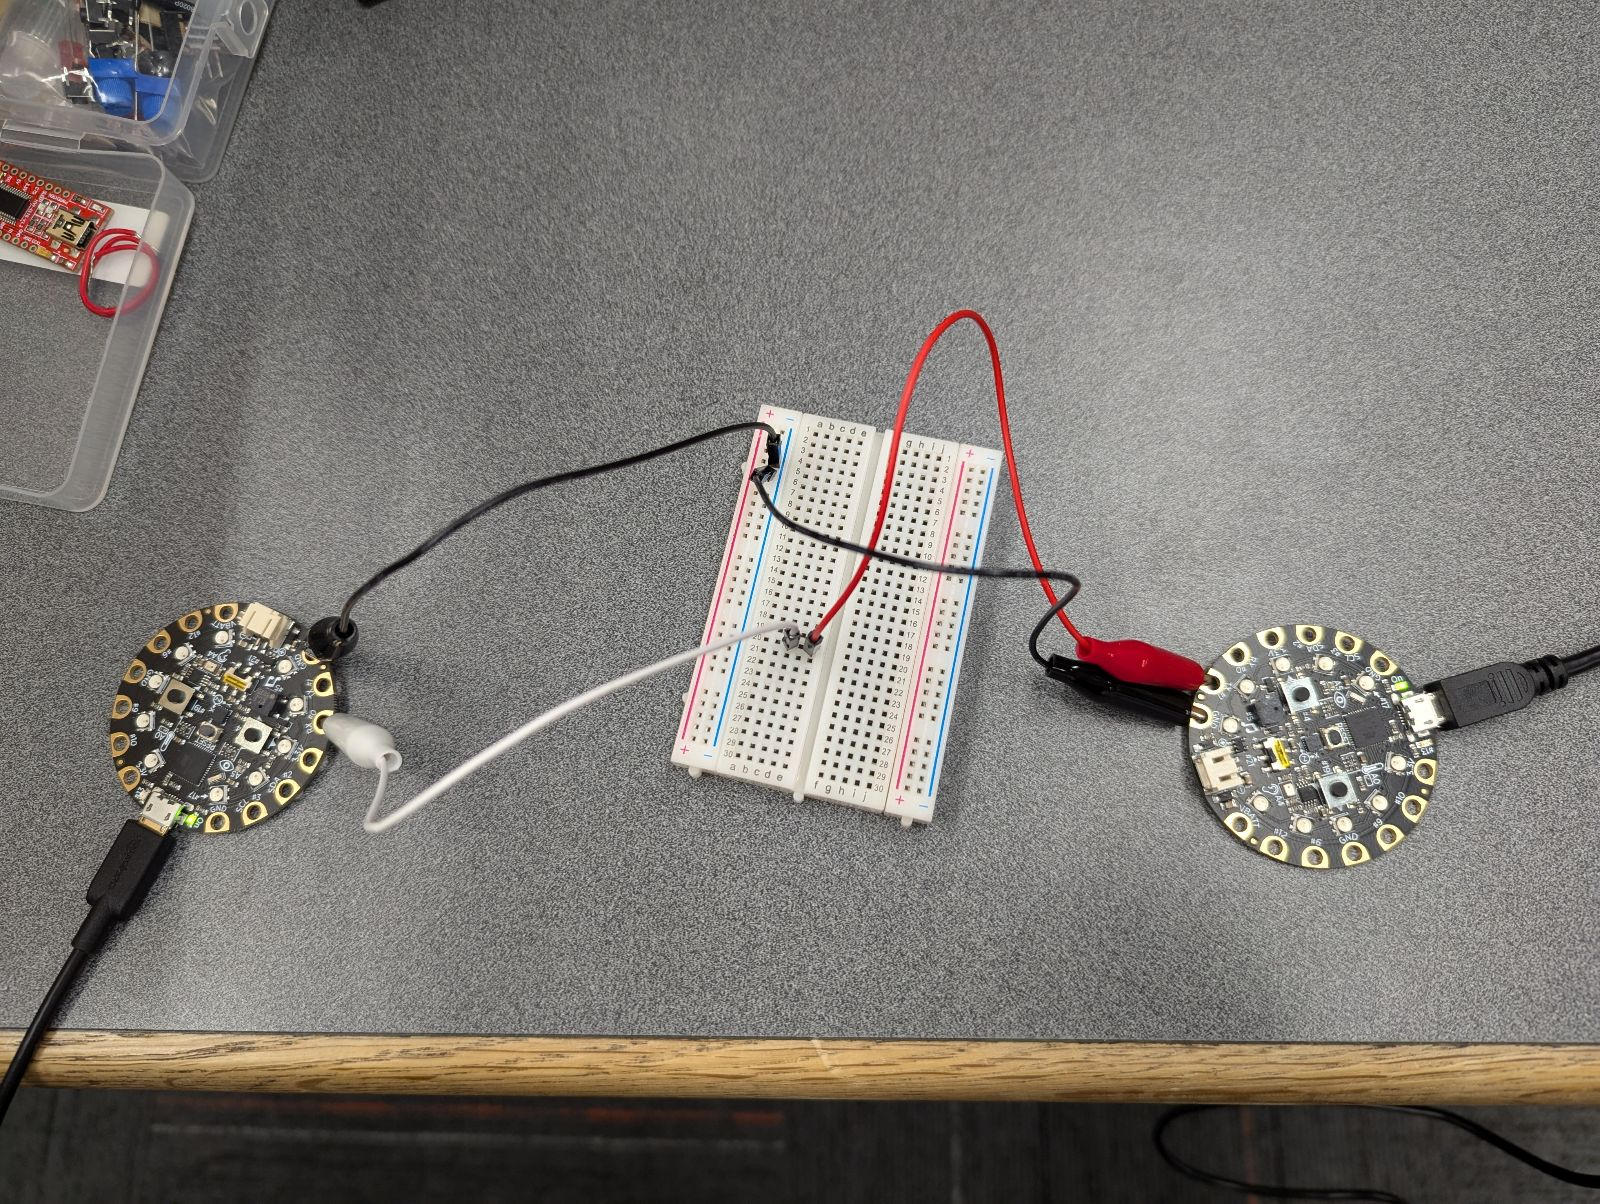
\includegraphics[width=\textwidth]{setup.jpg}
        \caption{Final Setup}
    \end{figure}
\end{minipage}
\hfill
\begin{minipage}{0.49\textwidth}
    \begin{figure}[H]
        \centering
        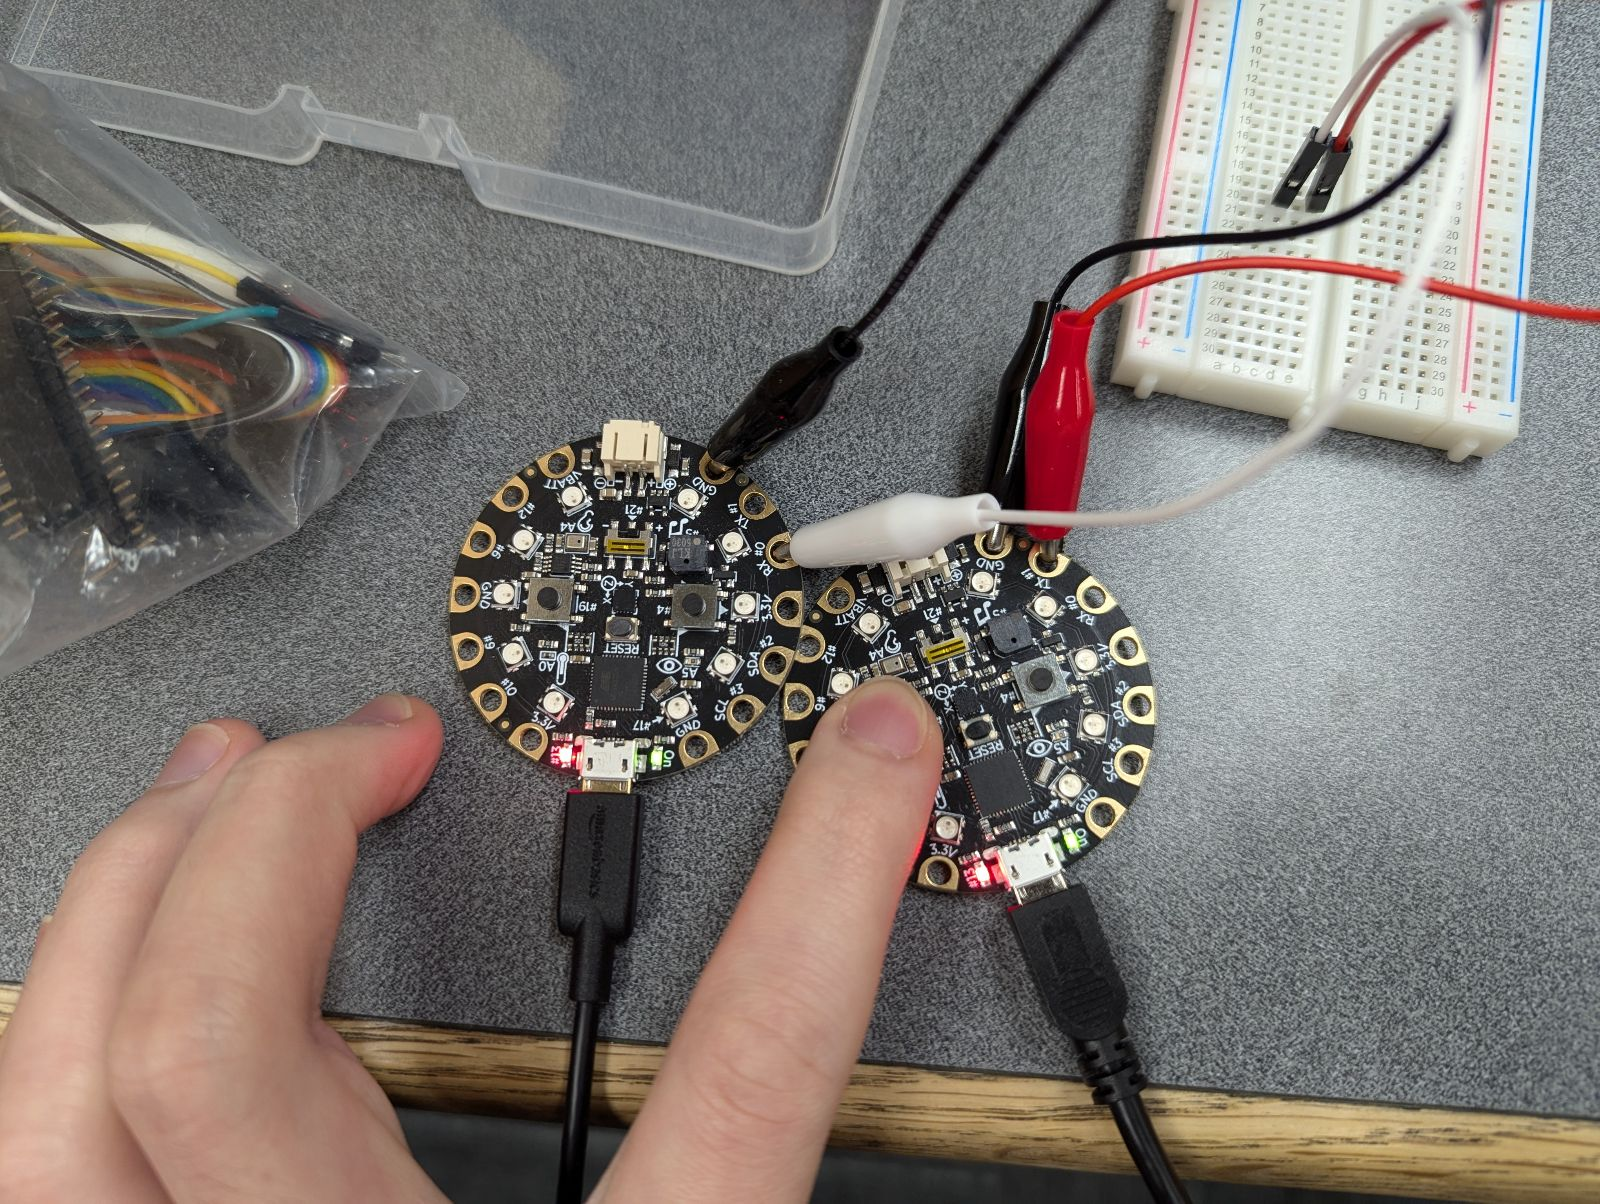
\includegraphics[width=\textwidth]{test.jpg}
        \caption{Testing}
    \end{figure}
\end{minipage}\\[0.5em]
{\Large \textbf{3. Conlcusion}}\\[0.5em]
    In this lab, we learned how to set up the USART on the ATMega32U4 microcontroller. We also learned how to set up the interrupt service routine for the USART receive interrupt. We also learned how to transmit data via USART and successfully fulfilled requirements and tasks in the lab manual. \\[1em]
{\Large \textbf{4. Code}}\\[0.5em]
{\Large \textbf{4.a Team A}}
\begin{verbatim}
            #include <Arduino.h>

            void setup() {
                UCSR1A = 0x00;          // UCSRA set as default. 
                UCSR1B = 0x00;          // UCSRB set as default.
                UCSR1C = 0x00;          // UCSRC set as default.

                UCSR1B |= (1<<RXEN1) |  // Enable receiver
                        (1<<TXEN1);     // Enable transmitter
                UCSR1C |= (1<<UCSZ10) |
                        (1<<UCSZ11);    // 8-bit data
                UBRR1 = 51; // UBRR1 = (fosc / (16 * Baud Rate)) - 1
                            //       = (8MHz / (16 * 9600)) - 1 = 51.08

                DDRF &= ~(1<<PF6);      // Right button PF6 as input
                DDRC |= (1<<PC7);       // Set PC7 as output
                PORTC &= ~(1<<PC7);     // Set LED to off

            }


            void loop() {
                // Team A
                if(PINF & (1<<PF6)){
                    PORTC |= (1<<PC7);  // Set LED to on
                    UDR1 = 0x31;        // Send 1
                } else {
                    PORTC &= ~(1<<PC7); // Set LED to off
                    UDR1 = 0x30; // Send 0
                }
            }
\end{verbatim}
{\Large \textbf{4.b Team B}}
\begin{verbatim}
                #include <Arduino.h>

                void setup() {
                    UCSR1A = 0x00; // UCSRA set as default. 
                    UCSR1B = 0x00; // UCSRB set as default.
                    UCSR1C = 0x00; // UCSRC set as default.

                    UCSR1B |= (1<<RXEN1) |  // Enable receiver
                    (1<<TXEN1) |            // Enable transmitter
                    (1<<RXCIE1)|            // Enable RX Interrupt
                    (1<<TXCIE1);            // Enable TX Interrupt
                    UCSR1C |= (1<<UCSZ10) |
                    (1<<UCSZ11);            // 8-bit data
                    UBRR1 = 51;             // UBRR1 = (fosc / (16 * Baud Rate)) - 1
                                            //       = (8MHz / (16 * 9600)) - 1 = 51.08

                    DDRF &= ~(1<<PF6);      // Right button PF6 as input
                    DDRC |= (1<<PC7);       // Set PC7 as output
                    PORTC &= ~(1<<PC7);     // Set LED to off

                    sei();
                }

                ISR(USART1_RX_vect){
                    if (UDR1 == 0x31){
                        PORTC |= (1<<PC7);
                    } else{
                        PORTC &= ~(1<<PC7);
                    }
                }

                void loop() {
                }
\end{verbatim}
\end{document}